\documentclass[a4paper, 12pt]{article}

%--------------------------------------------------------------------------
%	PACKAGES
%--------------------------------------------------------------------------
\usepackage[utf8]{inputenc}
\usepackage[OT1]{fontenc}
\usepackage{textcomp}
\usepackage[english]{babel}
\usepackage{amsmath, amssymb, amsthm, amsfonts}
\usepackage{mathtools}
\usepackage{nccmath}
\usepackage[linesnumbered, ruled]{algorithm2e}
\usepackage{fancyhdr}
\usepackage{lastpage}
\usepackage[left=2.5cm,right=2.5cm,top=2.5cm,bottom=2.5cm]{geometry}
\usepackage{numprint}
\usepackage{nicefrac}
\usepackage{dsfont}
\usepackage{gensymb}
\usepackage[shortlabels]{enumitem}
\usepackage{subcaption}
\usepackage{titling} % Customizing the title section
\usepackage{blindtext}
\usepackage{xcolor}
\usepackage{xurl}
\usepackage{hyperref} % For hyperlinks in the PDF
\usepackage{multicol}
\usepackage{microtype}
\usepackage{graphicx}
\usepackage{perpage}
\usepackage{afterpage}
\usepackage[round]{natbib}
\usepackage{usebib}
\usepackage[nottoc, numbib]{tocbibind} 
\usepackage[titletoc, title]{appendix}
\usepackage{graphicx}
\usepackage{float}
%--------------------------------------------------------------------------
%	TITLE PAGE
%--------------------------------------------------------------------------
\pretitle{\vspace{-3\baselineskip}\begin{center}\Huge\bfseries} % Article title formatting
\posttitle{\end{center}} % Article title closing formatting
\title{Genome-wide association study on coronary artery disease \vspace{0.3cm}} % Article title
\author{\smallskip
\large \textsc{Fahim Beck}}
\date{\vspace{-1.3cm}}
%--------------------------------------------------------------------------
%	OTHER SETTINGS
%--------------------------------------------------------------------------
\tolerance=10000 %Badbox errors
\hbadness=10000 %Badbox errors
\hfuzz=\maxdimen %ici nécessaire (Badbox errors)

\parindent=0cm %indentation réglé à 0cm
\setlength{\headheight}{15pt}
\setlength{\columnsep}{0.14cm}
\setitemize{itemsep=-1pt}
\MakePerPage{footnote}
\addto\captionsenglish{\renewcommand\contentsname{Table of Contents}}
\addto\captionsenglish{\renewcommand\bibname{References}}

% Cite title
\bibinput{references}
\newcommand{\citetitle}[1]{\hyperlink{cite.#1}{(\usebibentry{#1}{title}, \usebibentry{#1}{year})}}

% Inline code style
\definecolor{codegray}{gray}{0.9}
\newcommand{\code}[1]{\colorbox{codegray}{\texttt{\frenchspacing #1}}}
%--------------------------------------------------------------------------
%	FANCY SETTINGS
%--------------------------------------------------------------------------
\fancypagestyle{plain}{
  \renewcommand{\headrulewidth}{0pt}
  \fancyhf{}
  \fancyfoot[L]{\raisebox{-0.4\baselineskip}{
\includegraphics[width=0.15\textwidth]{images/EPFL.png}}}
  \fancyfoot[R]{\thepage /\pageref{LastPage}}
}

\rhead{Fahim Beck}
\lhead{}
\lfoot{\raisebox{-0.4\baselineskip}{
\includegraphics[width=0.15\textwidth]{images/EPFL.png}}}
\cfoot{}
\rfoot{\thepage /\pageref{LastPage}}
\pagestyle{fancy}
%--------------------------------------------------------------------------

\begin{document}

\maketitle

\section{Introduction and background}

Coronary artery disease (CAD) is one of the major causes of death worldwide. It causes a reduction in blood flow in the arteries of the heart through plaque formation (arteriosclerosis). There are many risk factors (smoking, alcohol, high blood cholesterol, obesity, etc). However, the heritability of this disease has been estimated between 40\% and 60\% \citep{heredity}. Hence the interest in carrying out a genome-wide association study.  

\subsection{Research questions and approaches}

The aim of this study is to identify associations among SNPs and the presence of CAD. For a GWAS, the four main steps are: (i) data pre-processing; (ii) new data generation; (iii) statistical analysis; and (iv) post-analytic interrogation. 

\subsection{Dataset}

The dataset comes from a GWA study of CAD (PennCATH) of the University of Pennsylvania Medical Center. It includes 3850 individuals enrolled between July 1998 and March 2003. A part of them of European ancestry were selected for genome-wide genotyping. Here, we consider anonymised data that includes 1401 individuals with genotype information over 861,473 SNPs. The clinical data gives information about the age, sex, HDL and LDL cholesterol, triglycerides and CAD status. 

\section{GWA analysis}

\subsection{Data pre-processing / QC steps}

Before starting the GWA analysis, it is necessary to proceed to some quality-control steps in order to remove (or "filter") poor quality data. Filtering will be done at two levels: at SNP and sample levels. Excluding SNPs that have been found to be of insufficient quality can be justified by several reasons, such as the large quantity of missing data, low variability, or genotyping errors. As for the exclusion of individuals, this may be due to missing data, sample contamination, correlation or other issues related to race, ethnicity or gender. 

\subsubsection*{SNP-level filtering -- part 1}

Here, the data are filtered according to two criteria: the call rate and the minor allele frequency (MAF). \\

The call rate is defined for a given SNP as the proportion of individuals for which the corresponding SNP information is not missing. In our case, we filter with a call rate of 95\%. All SNPs that have more than 5\% missing data will be removed. \\

As for the second criterion, we remove all SNPs for which the MAF is less than 1\%. Indeed, if a large majority of the participants have two copies of the major allele, then there will be little variability and the power of our statistical tests will be reduced, i.e. it will be more difficult to infer a significant relationship between the SNP and the trait studied. \\

After this step, we are left with 658,186 SNPs. Indeed, 203,287 SNPs were removed. 

\subsubsection*{Sample-level filtering}

Similar to what was done at the SNP level on the call rate criterion, we remove the individuals whose percentage of missing SNPs is more than 5\% (call rate is 95\%). \\

Then, a second criterion concerns heterozygosity. Under Hardy-Weinberg equilibrium (HWE), the probability of observing both alleles at a given SNP is $2p(1-p)$ where $p$ is the frequency of the dominant allele. We would therefore like to remove individuals with an inbreeding coefficient $|F| = (1-O/E) >0.1$, where $O$ and $E$ are respectively the observed and expected numbers of heterozygous SNPs. \\

Another problem concerns the relationship between individuals. In such studies, it is possible to unintentionally recruit two or more individuals from the same family. One measure to quantify relatedness is the identity by descent (IBD). An IBD kinship coefficient of more than 0.1 can reinforce the hypothesis that the pair in question is related. Before proceeding to this analysis, linkage disequilibrium (LD) pruning is applied with a threshold of 0.2. This will eliminate duplicates and other types of redundancy. It will also result in a lot of computational savings. This filtering reduces considerably the SNPs from 658,186 to 72,812. Then, the IBD analysis indicates that no pair suggests a family relationship. \\
With the same filtering, we consider a last aspect which is about ancestry. Here, we would like to remove individuals who are not part of an ethnic/racial group. For this, PCA helps us visualising the different ancestry groups according to the genetic information. The 72,812 SNPs are given as input for the PCA. Figure \ref{fig:PCA} shows a plot of the first principal component against the second one. \\

\begin{figure}[!ht]
\centering
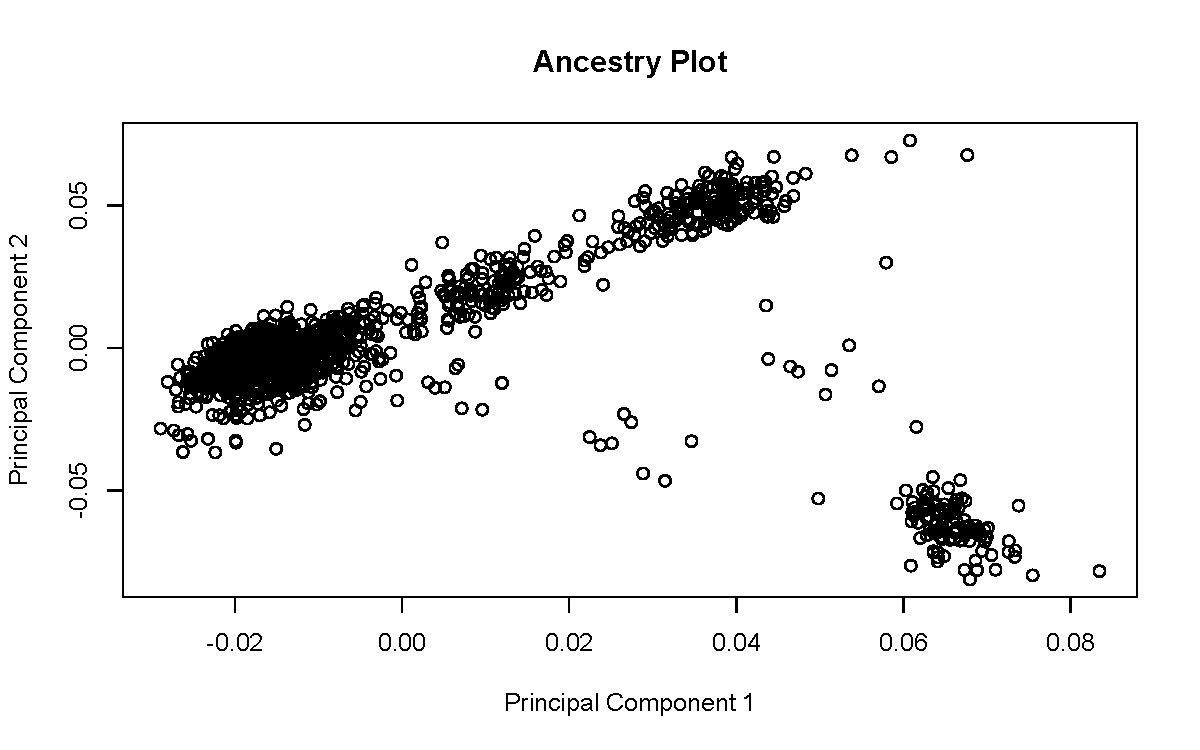
\includegraphics[width=0.8\textwidth]{../Plots/PCA}
\caption{Plot of PC1 against PC2 for representing individuals by ancestry groups based on their genetic composition.}
\label{fig:PCA}
\end{figure}

Visual inspection of this plot does not require removing more individuals. It should be noted that the PennCATH data has also been pre-filtered. 

\subsubsection*{SNP-level filtering -- part 2 (HWE)}

A final filtering at the SNP level consists of removing SNPs that violate HWE. These may indicate a genotyping error. To do this, SNPs whose HWE test statistic (obtained by a $\chi^2$ test between the observed and expected genotypes) has a $p$-value lower than $1 \times 10^{-6}$ in CAD controls are removed. This corresponds to 1,296 SNPs. This leaves 656,890 SNPs for association analysis. 

\subsection{Association / post-association analysis}


\newpage

\section{Conclusion}


\nocite{*}
\setcitestyle{numbers}
\bibliographystyle{abbrvnat}
\bibliography{references}

%\begin{appendices}
%	\section{Something}
%\end{appendices}

\end{document}
